\documentclass[11pt]{article}
\usepackage{amssymb}
\usepackage{amsmath}
\usepackage{amsfonts}
\usepackage{hyperref}
\usepackage{alltt}
\usepackage{graphicx}

\setlength{\textheight}{8.5in}          
\setlength{\textwidth}{6.0in}
\setlength{\headheight}{0in}
\addtolength{\topmargin}{-.5in}
\addtolength{\oddsidemargin}{-.5in}

\usepackage{concmath}
\usepackage[T1]{fontenc}

\title{MapReduce for Stampede}
\author{
  Sai Avala\\ 
  \href{mailto:sai.avala@utexas.edu}
          {sai.avala@utexas.edu}  \\ \\
  Sudheesh Katkam \\
  \href{mailto:sudheesh.katkam@utexas.edu}
          {sudheesh.katkam@utexas.edu}  }

\begin{document}
\maketitle
\newpage
\rule{6.0in}{.001in}
\tableofcontents
\newpage

\section{Introduction}
Most high performance computing systems are a connected cluster of inexpensive computers. These computers collectively solve computationally intensive problems, e.g. weather prediction. This distributed memory model allows for processors to run identical or different programs, each working on different chunks of problem/ data. This provides scalability: adding more processors to the system adds more units of computation. However, as there is no global memory for all processors, exchanging data becomes necessary, say near the borders of the data chunks. This communication is done explicitly through Message Passing Interface or MPI. Routines include Point-to-Point messages, collective messages, synchronization, etc. These routines are complex and programmers are required to learn the function signatures and the various parameters required. MApReduce for Stampede is a C++ library that provides an abstraction for programmers to focus on solving the problem rather than worry about the underlying communications among the processors. MARS is an abstraction over Boost.MPI which itself is an abstraction over MPI.

\subsection{MapReduce}
MapReduce is a programming paradigm that enables developers to take advantage of clusters that make the same operations on each element in a given dataset. With MapReduce, a developer can distribute data easily and apply the same computations without having to worry about the actual maintainence or synchronization. For our project, we decided to build a MapReduce API (MARS)for C++. As the end result, the developers will only need to know how to formulate their algorithm and our API will handle the actual distribution of the data and the ending reduction.

\subsection{Boost.MPI}
Boost.MPI is a library for message passing in high-performance parallel applications. Unlike communication in threaded environments or using a shared-memory library, Boost.MPI processes can be spread across many different machines, possibly with different operating systems and underlying architectures. It is a C++-friendly interface to the standard Message Passing Interface (MPI), the most popular library interface for high-performance, distributed computing. This library provides an interface to MPI that better supports modern C++ development styles, including complete support for user-defined data types and C++ Standard Library types.

\subsection{Problem}
Although Boost.MPI provides a good abstraction, it still involves knowing MPI. Boost.MPI, although an abstraction still uses similar MPI function calls, so the programming style is similar but provides a slightly higher level of programming compared to the standard MPICH2 or Open MPI.

\section{Setup}
\subsection{Constraints}
Given that we know that the MARS API will used so that the developer only needs to focus on formulating their algorithm instead of handling synchronization between processors, we had to make sure the MapReduce handled it for the developer. Since our API is meant for C++ developers, we used MPICH-2 (MPI) in order to maintain the computations across nodes within a cluster. As developers of the API we constrained the expectations of those who use this library to be able to write the actual computation that they would like to see on their data. For example, given a large list of numbers of size "n", the developer should understand what computation they want to be done on each element of the list. 
\subsection{Modeling MapReduce}
Our project, although universal, was designed to work with the Stampede Supercomputer Cluster. Earlier we stated that our MapReduce API will handle the distribution of data across multiple processes. To show how this is possible, let's list out a few definitions.
\begin{itemize}
  \item Master: A process that initially distributes the data and gathers the output after all the computations have completed
  \item Mapper: A set of processors which apply the user defined computation on the elements of the dataset. The Mapper returns a tuple of the key (the unique element in the dataset) and a value (occurrence, count, etc.).
  \item Reducer: A set of processors which reduce the tuples defined in Mapper and applies the user defined function that specifies how to reduce or combine the individually mapped out data. After reducing all the values associated with the common keys, the Reducer processes send the data back to Master, which then outputs the result.
\end{itemize}
\subsection{Formulation}
In order to use this API, we modeled the library such that the user needs to define the Mapper and Reducer. Assuming that the computation is the same on every element of the dataset, the Master process is what decides how to split the dataset to the rest of the processes. For this piece of the project we could not assume that each process will be given a single element in the dataset, otherwise the number of processes will be the size of the dataset, which is impossible to have. 
\newline 
\indent The Master process lets the user define how the dataset should be split. Furthermore, because we are assuming the computation on each element of the dataset is the same or independent, the user will define the map() function within the Mapper class. The map() function returns tuples of key (the element of the dataset) and the value, which is the value after applying the map() function. The user will also define the reduce() function within the Reducer class, which takes in each of the common keys and applies the reduce() function to congregate all the values to return a single key value pair.
\newline
\indent The Mapper class contains the map() function, which we assume applies a computation that is uniform across each element of the dataset. Essentially, if the data is a list \newline [1, 2, 3, 4], then the map() function could just add 1 to each element. The output key value pairs of the map() function could look like this [(1, 2), (2, 3), (3, 4), (4, 5)] where the value is the given element of the dataset incremented by one. Notice how because each computation is independent, we can distribute the data and let the map() function run in parallel across processes in Stampede.
\newline
\indent
The Reducer class contains the reduce() function, which takes in a list of common key value pairs, where the key is common, and then applies reduce() in order to aggregate the list of values into one single value. This new key value pair is then sent back to Master, who then handles how to output the result. Assume that you have a key value pairs list (key, [v1, v2 v3]), reduce() will return a (key, finalValue) and broadcast that back to Master.
%\subsubsection*{Phase 2}
%Work
%\subsubsection*{Phase 3}
%Testing
\section{Usage}
The classic example is to show how to use our MapReduce API in order to get a character count from a set of strings. Let's say that you have the String:
\begin{verbatim}
"Hey how is it going"
\end{verbatim}
Our end result should look like:
\begin{verbatim}
e 1
g 2
h 2
i 3
n 1
o 1
s 1
t 1
w 1
y 1
\end{verbatim}
In order to properly use this API, the user needs to define the Master class, the map() function in Mapper, and reduce() within Reducer. To make computations easier, we already split up the data for the user, but it is still helpful to look at a sample formulation:
\begin{verbatim}
class CharCountMapper : public Mapper<MK, MV, RK, RV> {

    virtual vector<RPAIR> map(vector<MPAIR> tuples) {
        return tuples;
    }
};

class CharCountReducer : public Reducer<RK, RV> {

    virtual RPAIR reduce(RK key, vector<RV> values) {
        RV sum = 0;
        for (int i = 0; i < values.size(); ++i) {
            sum += values[i];
        }
        return RPAIR(key, sum);
    }
};
\end{verbatim}
Since we have already split up the tuples in the data set, which is a string, our map() function will just output a character key and the initial value as 1. We use 1 as the default value because naturally that starting count number given an occurrence. After the map() function is applied to every item in the dataset, Master will go ahead and create a new pair such that all the common keys value pairs will be passed into reduce() as a single key and a list of values. reduce() in our case will taken in a key and list of values pair, sum up the occurrences, which is the list of values and then sends the final result back to Master.

Another example of the MARS framework is that the developer can easily use it in order to do a matrix multiplication. Given the input matrix and the code sample below, the developer can easily compute a matrix multiply.

\begin{verbatim}
class MatrixMapper : public Mapper<MK, MV, RK, RV> {

    virtual vector<RPAIR> map(vector<MPAIR> tuples) {
        vector<RPAIR> result;
        for (int i = 0; i < tuples.size(); ++i) {
            RK key = tuples[i].first;
            MV values = tuples[i].second;

            RV prods;
            for (int j = 0; j < values.size(); ++j) {
                int r = values[j].first;
                int c = values[j].second;

                prods.push_back(r * c);
            }

            result.push_back(RPAIR(key, prods));
        }

        return result;
    }
};

class MatrixReducer : public Reducer<RK, RV> {

    virtual RPAIR reduce(RK key, vector<RV> values) {
        int sum = 0;
        for (int i = 0; i < values.size(); ++i) {
            RV rv = values[i];

            for (int j = 0; j < rv.size(); ++j) {
                sum += rv[j];                
            }
        }

        RV result;
        result.push_back(sum);
        return RPAIR(key, result);
    }
};
\end{verbatim}
\section{Assumptions}
RK needs to be hashable. Enhancement: requires data to fit on one processor (master) which is sent to various  workers.

\section{Performance}
The original code for the MARS framework was built using blocking send() and recv() calls. This results in Master having to wait completely until all of the map() jobs have finished. By extending MARS to use nonblocking send() and recv() calls, we increased performance in communication among the processors.

Boost.MPI as stated earlier, abstracts the MPI framework to a certain amount. So, part of this discussion is to see how Boost usage affects the performance of the framework compared to just using explicit MPI function calls. According to the Boost.MPI framework, the speed difference is only slightly marginal. In fact, in Boost.MPI does not show any change that would affect the user of our MARS framework. As a result, using MPI or Boost.MPI is completely fine. A graph plotting out the performance of Boost.MPI and MPI in sending messages shows the similarity in performance (Boost documentation).

\hspace{-.2em}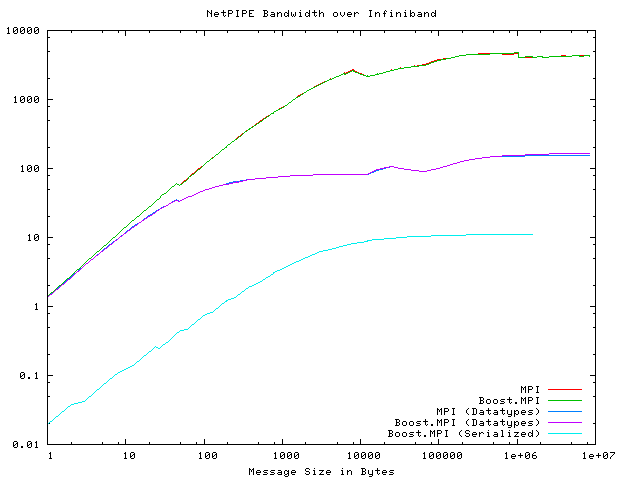
\includegraphics[scale=0.6]{boost_performance}

\section{Future Plans}
The current build of the MARS framework, assumes that the user will understand how the input data will be split to the processors. Making the user specify the data split is the next task to be abstracted. The current project requires that the developer input the dataset in a format understood by map() and reduce(). In the next build of the project, the framework will provide a higher level of development where the user will specify Input and Output classes. The user will provide the data as a text or csv file and Input will decide how to split the data. Likewise, when the MapReduce job completes, the results are sent to the Master process in which the Output class will handle the final manipulation of data - reorganizing and printing to file, etc.

\section{Conclusion}
MARS provides a MapReduce abstraction where the programmer is unaware of the underlying complexity of making MPI function calls. MARS lets the developer take advantage of clusters and computation on large datasets without them having to think about common issues with distributed programming: synchronization, sending, and receiving messages. MARS is a MapReduce framework for Stampede that lets the user focus on writing code for computations on the data.

\end{document}
